\documentclass{article}
\usepackage{graphicx}
\usepackage{listings}
\usepackage[left=2cm, right=2cm]{geometry}
\title{Hand-in 1}
\author{Michael Iversen}

% Default fixed font does not support bold face
\DeclareFixedFont{\ttb}{T1}{txtt}{bx}{n}{10} % for bold
\DeclareFixedFont{\ttm}{T1}{txtt}{m}{n}{10}  % for normal

% Custom colors
\usepackage{color}
\definecolor{deepblue}{rgb}{0,0,0.5}
\definecolor{deepred}{rgb}{0.6,0,0}
\definecolor{deepgreen}{rgb}{0,0.5,0}

\usepackage{listings}

% Python style for highlighting
\newcommand\pythonstyle{\lstset{
		language=Python,
		basicstyle=\ttm,
		morekeywords={self},              % Add keywords here
		keywordstyle=\ttb\color{deepblue},
		emph={MyClass,__init__},          % Custom highlighting
		emphstyle=\ttb\color{deepred},    % Custom highlighting style
		stringstyle=\color{deepgreen},
		showstringspaces=false
}}

% Python environment
\lstnewenvironment{python}[1][]
{
	\pythonstyle
	\lstset{#1}
}
{}


\begin{document}
\maketitle
\section*{PART I: Logistic Regression}
	\subsection*{Code}
	\subsubsection*{Summary and results}
	Figure \ref{fig:logreg} shows the insample error as a function of epochs when applying the mini-batch gradient descent algorithm.
	After $50$ epochs the insample error is $E_\mathrm{in} = 0.08$ and test error $E_\mathrm{test} = 0.11$.
	\begin{figure}
		\centering
		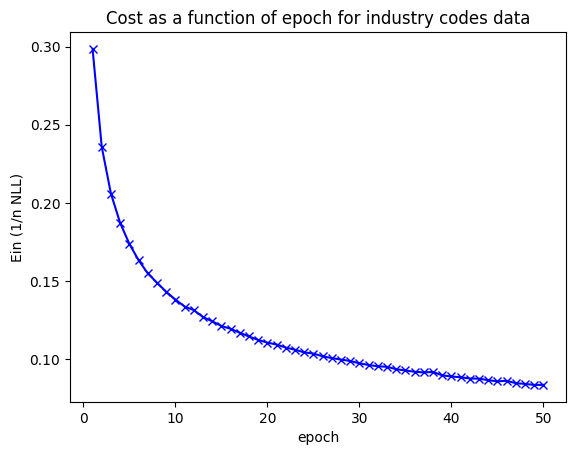
\includegraphics[width=0.5\textwidth]{logreg_text_cost_per_epoch.png}
		\caption{Insample error as a function of number of epochs.}
		\label{fig:logreg}
	\end{figure}
	\subsubsection*{Actual code}
	The code below shows my implementation of the method ``cost\_grad''
	The docstring is omitted to simplify the code snippet.
	\begin{python}
def cost_grad(self, X, y, w):
	cost = 0
	grad = np.zeros(w.shape)
	
	n = X.shape[0]  # Number of data points
	d = X.shape[1]  # Number of features
	for i in range(n):
		arg = 0    # Argument of exp(...): -y_i * w^T @ x_i
		for j in range(d):
			arg += -y[i] * w[j] * X[i, j]
		cost += np.log(1 + np.exp(-arg))
	cost /= n
	
	for k in range(d):
		for i in range(n):
			arg = 0
			for j in range(d):
				arg += -y[i] * w[j] * X[i, j]
			grad[k] += y[i] * X[i, k] * logistic(arg)
		
	grad /= n

	assert grad.shape == w.shape
	return cost, grad
	\end{python}
	The same problem can be solved concisely using broadcasting of numpy arrays.
	\begin{python}
def cost_grad(self, X, y, w):
	cost = np.mean(np.log(1 + np.exp(-X @ w * y)))
	grad = np.mean(-y * X.transpose() * logistic(-X @ w * y), axis=1)
	assert grad.shape == w.shape
	return cost, grad
	\end{python}
	Since the first implementation is more transparent than the second, we will use this implementation to explain the time complexity in the next section.
	The code below shows my implementation of the fitting method.
	\begin{python}
def fit(self, X, y, w=None, lr=0.1, batch_size=16, epochs=10):
	if w is None:
		w = np.zeros(X.shape[1])
	history = []
	for _ in range(epochs):
		permutation = np.random.permutation(np.arange(X.shape[0]))
		X_permuted = X[permutation, :]
		y_permuted = y[permutation]
		for idx_start in np.arange(0, X.shape[0], batch_size):
			idx_stop = idx_start + batch_size
			X_batch = X_permuted[idx_start:idx_stop, :]
			y_batch = y_permuted[idx_start:idx_stop]
			_, grad = self.cost_grad(X_batch, y_batch, w)
			w += -lr * grad
		cost, _ = self.cost_grad(X, y, w)
		history.append(cost)

	self.w = w
	self.history = history
	\end{python}
\subsection*{Theory}
	\subsubsection*{Time complexity}
	We investigate the running time to compute the cost and gradient in ``cost\_grad''.
	We start by studying the running time of computing the cost.
	The first for-loop executes the inside code $n$ times and the next for loop executes $d$ times.
	Inside the for-loops, the multiplication $-y[i]*x[j]*X[i,j]$ and evaluation of $np.log(1 + np.exp(-arg))$ takes constant time.
	Therefore, the time complexity of computing the cost is $O(nd)$.
	
	Computing the gradient is more complicated. 
	The first, second and third for-loops execute the inside code respectively $d$, $n$ and $d$ times.
	All calculations in the for-loops takes constant time.
	Therefore, the gradient is calculated in $O(nd^2)$ time.

	We investigate the running time of the mini-batch gradient descent algorithm.
	The outermost for-loop executes the inside code $epochs$ times.
	Moving inside this for-loop, the permutation of $X$ and $y$ takes place in $O(n)$ time.
	The next for-loop executes the inside code $\lfloor n/batch\_size \rfloor$ times.
	Inside this for-loop, computing the gradient takes $O(nd^2)$ time.
	Finally, computing the cost after each epoch also takes $O(nd^2)$ time because I am also (without purpose) computing the gradient.
	In total, the gradient descent algorithm has time complexity $O(epochs\cdot n^2 d^2/batch\_size)$.
	
	The algorithm can be optimized by only computing the gradient (not the cost) in the innermost for-loop and only computing the cost (not the gradient) in the outermost for-loop. 
	However, this optimization does not change the time-complexity. 
	
	\subsubsection*{Sanity check}
	If the pixels in all images are randomly permuted (in the same way), then I expect the classifier to perform as well as without the permutation.
	If the features are simply the rgb-values of all pixels, then our model does not use any locality information of the data and the performance is not affected by destroying the locality information by a permutation.
	If $\omega$ is an optimal model without the permutation, then $\omega' = \mathrm{P}(\omega)$ is an optimal model for the permuted data where $\mathrm{P}(\cdot)$ is the permutation of the pixels.
	
	\subsubsection*{Linearly separable data}
	When the data is linearly separable, there exists a model $\omega$ which perfectly classifies all data.
	The gradient descent algorithm finds this optimal model unless it gets stuck in a local minima.
	
\section*{PART II: Softmax}
\subsection*{Code}
\subsection*{Theory}	
	
\end{document}